\documentclass[12pt,a4paper]{article}
\usepackage{times}
\usepackage{durhampaper}
\usepackage{array}
\newcolumntype{P}[1]{>{\centering\arraybackslash}p{#1}}
\usepackage{url}
\usepackage{amsmath}
\usepackage{harvard}
\usepackage[utf8x]{inputenc}
\usepackage{wrapfig}
\usepackage{booktabs}
\usepackage{enumitem}
\usepackage{graphicx}
\usepackage{float}
\usepackage{multirow}
\usepackage{titlesec}
\setcounter{secnumdepth}{4}
\usepackage{cite}
\citationmode{abbr}
\bibliographystyle{plain}



\title{An Analysis of Machine Learning and Deep Learning Techniques for Detecting Sarcasm in Online Text}
\author{} % leave; your name goes into \student{}
\student{Molly Hayward}
\supervisor{Dr Noura Al-Moubayed}
\degree{BSc Computer Science}

\date{}

\begin{document}
	
\maketitle

\begin{abstract}
\\ \indent \textbf{Context / Background --} 
Sarcasm is a unique form of language that cannot be interpreted at surface-level. Detecting sarcasm proves a significant challenge for traditional sentiment analysers and humans alike. This highlights the scope for innovative machine learning and deep learning solutions to this ill-structured problem.

\indent \textbf{Aims --} Despite the challenges in this domain, this ultimate aim of this project is to produce a tool that can detect sarcasm in online text with a \textit{high degree} of accuracy. 

\indent \textbf{Method --} State-of-the-art contextualised word embeddings (ElMo vectors) and deep learning classification models are used to realise this aim.

\indent \textbf{Results --} Through extensive experimentation, we show that

\indent \textbf{Conclusions --} In summary, we conclude that

%This section should not be longer than half of a page, and having no more than one or two sentences under each heading is advised. Do not cite references in the abstract.
\end{abstract}

\begin{keywords}
Machine learning, Deep learning, Sarcasm Detection, Sentiment, Classification
\end{keywords}


\section{Introduction}
\noindent Sarcasm is a complex linguistic phenomenon, which when present in text indicates that the literal interpretation differs from the implied meaning. Sarcasm is prevalent in online user-generated content, and poses a significant challenge within the field of natural language processing, specifically within sentiment analysis, as it inverts the sentiment-polarity of a positive or negative utterance. Sentiment analysis is the task of deducing the sentiment polarity of text - typically whether the author is in favour of, or against, a certain subject. It is increasingly common for organisations to use sentiment analysis in order to gauge public opinion on their products and services; however, classic sentiment analysers cannot deduce the implicit meaning of sarcastic text and will wrongly classify the author's opinion. Hence, any tool that strives to accurately determine the meaning of user-generated text must be capable of detecting sarcasm. The phenonmenon of sentiment incongruity often lies at the heart of sarcasm, therefore advancements in automatic sarcasm detection research have the potential to vastly improve the sentiment analysis task.

\subsection{Problem Background}
\noindent As sarcasm is multi-faceted, this makes its detection a unique and interesting challenge. It can be both explicit and implicit; oftentimes, contextual cues are more powerful indicators of sarcasm than the words themselves. However we often lose this context, and hence the sarcastic undertones, in transcription. Consider the scenario where a person is congratulated on their hard work, despite the obviousness of them having not worked hard at all. Or perhaps a customer thanking a waiter for the delicious food, even though they sent it back to the kitchen. In isolation, the speech is not enough to convey the sarcastic intent. Furthermore, even humans struggle to consistently recognise sarcastic intent; due in part to the lack of an all-encompassing, universal definition of sarcasm. In a 2011 study, Gonz{\'a}lez-Ib{\'a}nez et al. \cite{gonzalez2011identifying} found low agreement rates between human annotators when classifying statements as either sarcastic or non-sarcastic, and in their second study, three annotators unanimously agreed on a label less than 72\% of the time. Truly, the existence of sarcasm can only be conclusively affirmed by the author. Additionally, developmental differences such as autism, as well as cultural and societal nuances cause variations in the way different people define and perceive sarcasm.

These factors make sarcasm detection an extremely complex task for both humans and computers. Despite this, \textit{most} humans can recognise sarcastic intent \textit{most} of the time. We strive to replicate this performance, or even perhaps improve upon it, in order to move towards a more concrete definition of what \textit{makes} a statement sarcastic. This highlights the scope for automating this process, and the need for an innovative solution.

Early rule-based approaches introduced the idea that the sentiment contained within text can be indicative of sarcasm, although exploring these sentiment features using more complex machine learning and deep learning architectures is a novel approach to the problem.

\subsection{Research Questions and Objectives}
\noindent The \textbf{research questions} guiding this project are as follows --\\
\indent \textit{- Do deep learning techniques perform better than machine learning approaches?}\\ 
\indent \textit{- Can we improve the solution by incorporating sentiment features?}\\ 
\indent \textit{- Can a custom model identify which linguistic cues correlate more to sarcastic labels?}\\

\noindent The following objectives are designed to address these specific research questions, and are divided into three categories depending on their priority level and difficulty.

The \textbf{minimum} objectives of this project are to evaluate, compare and clean high-quality datasets, as well as to employ machine learning models and evaluate the effectiveness of these architectures on our chosen datasets. We found that a logistic regression model trained on ElMo vectors performed best for all three datasets, achieving $F_{1}$ scores of 84.6\%, 81.3\% and \_\%. 

The \textbf{intermediate} objectives of this project are to experiment with and evaluate deep learning models on the chosen datasets, and to determine which is the best performing solution. Additionally, we evaluate the model against unseen data. This is achieved by ...

The \textbf{advanced} objectives of this project are to implement an attention-based deep neural network in order to identify words that correlate more to sarcastic labels, in order to produce a visualisation of attention words. We implement a custom attention layer using keras, and apply our trained model to a number of sentences to illustrate its effectiveness.

This is achieved by...




%This section briefly introduces the general project background, the research question you are addressing, and the project objectives.  It should be between 2 to 3 pages in length.\\%

\newpage
\section{Related Work}
\noindent In this section, we compare classification model architectures used specifically in sarcasm detection research, as well as techniques that have seen success in other natural language processing (NLP) classification tasks. In most approaches, sarcasm detection is treated as a binary classification problem, in which text is grouped into two categories - sarcastic and non-sarcastic. It is otherwise treated as a multi-class problem where the extent to which a statement is sarcastic is ranked on a discrete scale, e.g. 1 to 5. 
In similar studies, the terms irony and sarcasm are often used interchangeably \cite{tsur2010icwsm}. For clarity, an overview of their definitions are given in figure 1. Both definitions capture the humourous intent in both sarcasm and irony, however sarcasm extends this definition to include the potential for criticism - often present in opinion-based content such as product reviews.\vspace{-10pt}

\begin{center}
	\textbf{Figure 1}: Comparison of definitions of Irony and Sarcasm\vspace{-10pt}
\end{center}
\begin{center}
\begin{tabular}{p{1.5cm}p{13cm}}
	\hline
	\textbf{Term} & \textbf{Definition}\\
	\hline\hline
	Irony & The use of words that are the opposite of what you mean, as a way of being funny.
	\footnotemark[1]\\
	\hline
	Sarcasm & The use of remarks that clearly mean the opposite of what they say, made in order to hurt someone's feelings or to criticize something in a humorous way.\footnotemark[2]\\
	\hline
\end{tabular}\\
\end{center}\vspace{-10pt}
\footnotetext[1]{www.dictionary.cambridge.org/dictionary/english/irony}
\footnotetext[2]{www.dictionary.cambridge.org/dictionary/english/sarcasm}

\subsection{Traditional Classifiers}\vspace{-10pt}
\noindent A number of simple linguistic approaches have been used in previous research. One such class of na\"{i}ve approaches is \textit{rule-based}, where text is classified based on a set of linguistic rules. Maynard and Greenwood (2014) \cite{maynard2014cares} proposed that the sentiment contained in hashtags can indicate the prescence of sarcasm in tweets, such as \#notreally in the example "I love doing the washing-up \#notreally". They used a rule-based approach, whereby if the sentiment of a tweet contradicts that of the hashtag, it is labelled sarcastic. They reported an $F_{1}$ score of 91.03\% on a random sample consisting of 400 tweets. 

Riloff et al. (2013) \cite{riloff2013sarcasm} sarcasm is described as a contrast between positive sentiment and negative situation. This description is leveraged by Bharti et al (2015) \cite{bharti2015parsing}, which presents two rule-based approaches to sarcasm detection. The first approach identifies sentiment bearing situation phrases, classifying the phrase as sarcastic if the negative situation is juxtaposed with a positive sentiment phrase. Rule-based techniques are fairly primitive when compared to their modern, deep learning counterparts, as each ruleset must be generated manually and for each dataset.

\subsection{Machine-Learning Classifiers}\vspace{-10pt}
\noindent A machine-learning algorithm can learn patterns that are associated with sarcastic and non-sarcastic data. This allows it to classify unseen text into these categories without the need for a static linguistic rule set. If the training data is high-quality and plentiful, or an effective unsupervised-learning algorithm is used, then the model can begin to make accurate predictions. There are a number of commonly used architectures of machine-learning classifiers, including Na\"{i}ve Bayes, Support Vector machines (SVMs) and logistic regression based classifiers. Although, not all approaches fit neatly into these categories.

Tsur et al. (2010) \cite{tsur2010icwsm} proposed a novel semi-supervised algorithm, \textit{SASI}, for sarcasm identification; trained on a small balanced seed of 160 reviews (80 sarcastic and 80 non-sarcastic) from a corpus of 66000 human-annotated Amazon product reviews. In order to mimic the ambiguous and spectral nature of sarcasm, a discrete score between 1 (non-sarcastic) and 5 (definitely sarcastic) is assigned to each sentence; scores of 3 and higher indicate sarcasm. Syntactic and pattern-based features are extracted and fed to a classifier which utilises a strategy similar to k-nearest neighbor (kNN), whereby a sarcasm score is assigned to an unseen vector based upon the weighted average of the k-nearest neighbors in the training set. They reported an $F_{1}$ score of 82.7\% on the binary classification task

Na\"{i}ve Bayes classifiers are supervised algorithms that use bayes theorem to make predictions. Reyes et al. (2013) \cite{reyes2013multidimensional} used a na\"{i}ve bayes and decision trees algorithm in order to detect irony which is closely related to sarcasm. They experimented with balanced and unbalanced distributions (25\% ironic tweets and 75\% other), achieving an F-score of 0.72 on the balanced distribution, dropping to 0.53 for the inbalanced distribution. In a similar vein, Barbieri et al. (2014) \cite{barbieri2014modelling} used random forest and decision tree classifiers, also for the detection of irony. They used six types of features in order to represent tweets, and recorded results over three categories of training data - education, humor and politics.

Support Vector Machines (SVM), can be effective when smaller amounts of training data are available, however they require more computational resources than na\"{i}ve bayes. SVMs use kernel functions to draw hyperplanes dividing a space into subspaces. Gonz{\'a}lez-Ib{\'a}nez et al\. (2011) \cite{gonzalez2011identifying} used two classifiers, support vector machine with sequential minimal optimisation, as well as logistic regression. Their best result was an accuracy of 0.65, achieved with the combination of support vector machine with sequential miniminal optimisation and unigrams. \textit{Pt{\'a}{\v{c}ek et al. (2014)}} \cite{ptavcek2014sarcasm} also used support vector machine and Maximum Entropy classifiers. They also performed classification on balanced and inbalanced distributions.

\subsection{Deep-Learning Classifiers}\vspace{-10pt}
Deep neural networks (DNNs) are increasingly being used in text classification tasks \cite{zhang2015character, poria2016deeper}. Though there are many forms of DNN, two commonly used architectures are Recurrent Neural Networks (RNNs) and Convolutional Neural Networks (CNNs). Oftentimes, deep neural networks require a lot more training data than machine learning algorithms, but have been shown to produce state-of-the-art results in several domains.

%https://arxiv.org/pdf/1703.03091.pdf



One particularly interesting technique is the \textit{Hierarchical Attention Network (HAN)} defined in Yang et al. (2016) \cite{yang2016hierarchical} - an attention-based LSTM. The intuition is that certain words and sentences in a document contribute more to its overall meaning, and this is highly context dependent. They included one attention mechanism at word-level and another at sentence-level, and this allowed them to determine which words and phrases correlate more to certain labels. Using a similar approach in the domain of sarcasm may allow me to highlight the attention-words that are strongly influence the level of sarcasm. A similar technique was applied in \textit{Ghosh et al. 2018)} \cite{ghosh2018sarcasm} where they concluded that emoticons such as ':)' and interjections e.g. "ah", "hmm" correspond with highly weighted sentences. Gated Recurrent Units (GRUs) are another type of RNN used to overcome the vanishing gradient problem.  \textit{Zhang et al. (2016)} \cite{zhang2016tweet} used a bidirectional gated RNN to capture local information in tweets, as well as a pooling neural network to extract context from historic tweets, achieving 78.55\% accuracy.

Convolutional Neural Networks allow us to extract higher-level features, and they are based on the mathematical operation of convolution. \textit{Zhang et al. (2015)}  \cite{zhang2015character} explored the used of character-level convolutional neural networks for text classification. This network consists of 6 convolutional layers and 3 fully-connected layers. They found that it showed better peformance on raw texts such as an Amazon product review corpus. CNNs have been previously used in sarcasm detection. For example, \textit{Poria et al. (2017)} \cite{poria2016deeper} describes a convolutional neural network (CNN) for sarcasm detection. \\


%This section presents a survey of existing work on the problems that this project addresses.  it should be between 2 to 4 pages in length.  The rest of this section shows the formats of subsections as well as some general formatting information for tables, figures, references and equations. Note that the whole report, including the references, should not be longer than 20 pages in length.  The system will not accept any report longer than 20 pages.  It should be noted that not all the details of the work carried out in the project can be represented in 20 pages.  It is therefore vital that the Project Log book be kept up to date as this will be used as supplementary material when the project paper is marked.  There should be between 10 and 20 referenced papers---references to Web based pages should be less than 10\%.



%The font used for the main text should be Times New Roman (Times) and the font size should be 12.  The first line of all paragraphs should be indented by 0.25in, except for the first paragraph of each section, subsection, subsubsection etc. (the paragraph immediately after the header) where no indentation is needed.


%In general, figures and tables should not appear before they are cited.  Place figure captions below the figures; place table titles above the tables.  If your figure has two parts, for example, include the labels ``(a)'' and ``(b)'' as part of the artwork.  Please verify that figures and tables you mention in the text actually exist.  make sure that all tables and figures are numbered as shown in Table \ref{units} and Figure 1.
%sort out your own preferred means of inserting figures


%The list of cited references should appear at the end of the report, ordered alphabetically by the surnames of the first authors.  References cited in the main text should use Harvard (author, date) format.  When citing a section in a book, please give the relevant page numbers, as in \cite[p293]{budgen}.  When citing, where there are either one or two authors, use the names, but if there are more than two, give the first one and use ``et al.'' as in  , except where this would be ambiguous, in which case use all author names.


%You need to give all authors' names in each reference.  Do not use ``et al.'' unless there are more than five authors.  Papers that have not been published should be cited as ``unpublished'' \cite{euther}.  Papers that have been submitted or accepted for publication should be cited as ``submitted for publication'' as in \cite{futher} .  You can also cite using just the year when the author's name appears in the text, as in ``but according to Futher \citeyear{futher}, we \dots''.  Where an authors has more than one publication in a year, add `a', `b' etc. after the year.

\section{Solution}
\noindent This project addresses a binary classification problem, aiming to determine if an unseen snippet of text is sarcastic or non-sarcastic. Our sarcasm detection tool employs trained classification models which form  predictions based on the knowledge gained from features encountered during training. Developing highly accurate classification models remains the greatest challenge in this project, therefore it is the central focus of our solution. Model peformance is strongly dependent on the data pre-processing and feature extraction techniques employed, as well as the choice of model architecture and training procedures. 

In our solution, high quality datasets are first collected and pre-processed. During feature extraction, the textual training data is transformed into numerical vectors and these features are used to train a classification model. The trained classifier is then carefully evaluated in order to account for potential overfitting. The following figure outlines the model pipeline, and each of these stages are further addressed in the remaining sections.



\begin{center}
	\textbf{Figure \_:} Overview of the solution
\end{center}
\begin{center}
	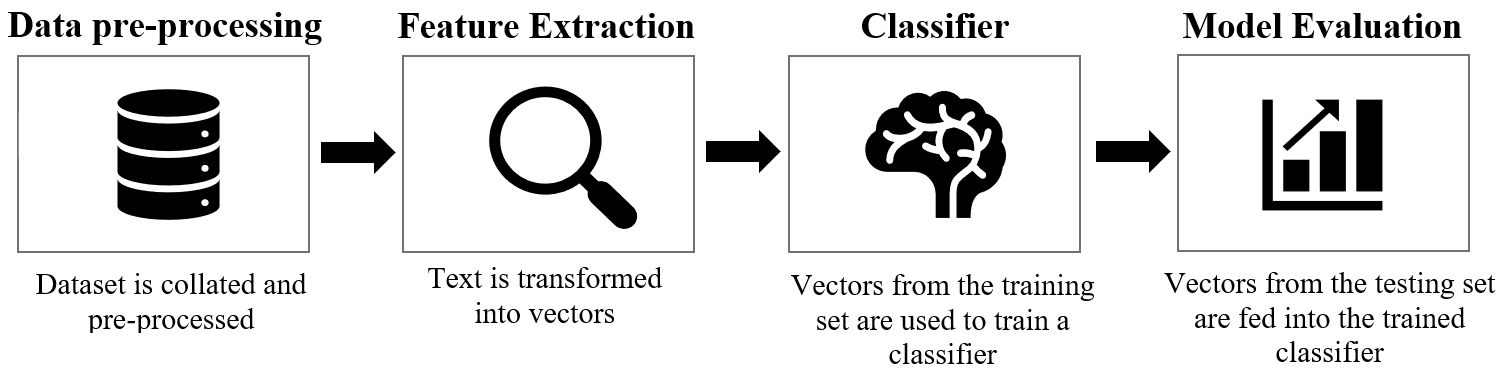
\includegraphics[width=0.8\textwidth]{Images/modelpipeline2.png}
	\label{Model Pipeline}
\end{center}

\subsection{Implementation Tools}
\noindent This project is majoritively written in \textbf{Python}, as it has an abundance of open-source libraries well-suited to machine learning and deep-learning tasks. Additionally, Python is very readable, making it easy for others to interpret, test and reproduce code. We use \textbf{pandas} for manipulating the datasets, as it provides functionality for applying functions globally across the dataset. We use \textbf{pickle} to store the vectorised datasets in memory. Vectorisation is a costly process, therefore writing the files to memory reduces long-term time demands during the experimentation and testing phases. We also  incorporate \textbf{SpaCy} when cleaning and tokenising the data.

In terms of \textit{classification}, we implement most of the machine learning architectures using \textbf{scikit-learn} - an open-source machine learning library. For constructing deep learning models, we use \textbf{keras}, as its modular structure allows for extensive experimentation and simplifies tweaking of model architectures.
\newpage
\subsection{Datasets}
\vspace{-4.2pt}\noindent We utilise three publically available datasets, and a statistical analysis of their properties is provided in \textit{figure \_}. This includes the number of instances in the dataset, the average number of tokens per instance and a benchmark score where the dataset was used in the original paper to train one or more classifiers. This data is collected from multiple domains and online platforms, including Twitter, Amazon, and online news outlets; providing broad coverage of sarcasm usage in both formal and informal media. \vspace{-4.2pt}


\begin{enumerate}[leftmargin=0cm]
	\item \textbf{News Headlines Dataset For Sarcasm Detection} - \textit{Misra et al. (2019)} \cite{misra2019sarcasm} collected thousands of news headlines from two sources - \textit{The Onion} \footnote{www.theonion.com} (renowned for posting satiricial news) and \textit{The Huffington Post} \footnote{www.huffpost.com}. News headlines are written formally, hence there is little noise in this dataset due to the absence of erroneous spelling. These headlines are self-contained, unlike tweets which may be in response to another tweet thereby excluding necessary context. Misra et al. (2019) \cite{misra2019sarcasm} used a hybrid neural network architecture and achieved an \textit{accuracy} of 0.897.\vspace{-4.2pt}
	
	\item \textbf{Sarcasm Amazon Review Corpus} - \textit{Filatova (2012)} \cite{filatova2012irony} used crowdsourcing to collect Amazon reviews, human-labelled by 5 annotators. The number of stars given to a review, as well as the title and content are provided. These reviews are typically longer than the average tweet, which is capped at 280 characters. The author's punctuation and spelling is preserved, therefore this data is very messy. This is the smallest of the three datasets. This dataset was not used by its compilers for classification, hence there is no score available for comparison.\vspace{-4.2pt}
	
	\item \textbf{Pt\'a\v{c}ek et al. (2014)} - One of three datasets collated in \textit{Pt\'a\v{c}ek et al. (2014)} \cite{ptavcek2014sarcasm}, we use a balanced dataset of 100000 English tweet ids, whereby the original tweet must be scraped using the Twitter API. Of this original corpus, 17.28\% of the original tweets remain available to access on Twitter, therefore all others are omitted from the compiled dataset. This dataset is messy, as sarcastic instances are those that include \textit{\#sarcasm}, and non-sarcastic instances are selected arbitrarily from the set of all other tweets. Hence, some of the sarcastic instances may not be sarcastic, and some non-sarcastic instances may be sarcastic. We take a subset of the remaining tweets (7500 from each class) to form a smaller balanced corpus. Pt\'a\v{c}ek et al. (2014) \cite{ptavcek2014sarcasm} achieved an $F_{1}$ score of 0.947.
\end{enumerate}

% For example, we avoid using datasets containing tweet ids, whereby the original tweet must be scraped using the Twitter API. A small portion of the original tweets are no longer available on twitter, therefore this does not make for a fair comparison between our results and the results of the source study.


\begin{center}
	\textbf{Figure -}: Statistical breakdown of the datasets used in this project \\
	\vspace{3pt}
	\begin{tabular}{P{3.3cm}P{2.6cm}P{2.5cm}P{2.2cm}P{3.4cm}}
		\hline
		\textbf{Dataset} & \textbf{Dataset Size} & \textbf{Composition}* & \textbf{Avg. tokens} & \textbf{Benchmark Score}\vspace{1pt}\\
		\hline
		News Headlines & 28619 & \begin{tabular}{c@{}@{}@{}} pos: 47.6\% \\ neg: 52.4\% \end{tabular} &  11.2 & 0.897\\
		\hline
		Amazon Reviews & 1254 & \begin{tabular}{c@{}@{}@{}} pos: 34.9\% \\ neg: 65.1\% \end{tabular} &  276.4 & N/A \\
		\midrule
		Twitter Data & 17280 & \begin{tabular}{c@{}@{}@{}} pos: 50.4\% \\ neg: 49.6\% \end{tabular} &  19.8 & 0.947 \\
		\hline
	\end{tabular}
\end{center}
\vspace{-7pt}
*\textit{pos} indicates positive instances (sarcastic) and \textit{neg} indicates negative instances (non-sarcastic)\\


\noindent The selected datasets were chosen due to their size, cleanliness and composition. Each of the selected datasets are sufficiently large enough to provide a representative view of their respective data sources without exceeding the available computational resources. In addition, these approximately balanced datasets are preferable to unbalanced datasets; despite the infrequent usage of sarcasm in real-life conversations. We can achieve 95\% accuracy when training a classifier on an unbalanced binary dataset where the class distribution is 95\% to 5\%, simply by annotating each datapoint with the majority class label. As most machine learning algorithms are designed to optimise overall accuracy, it is important to provide it with approximately equal amounts of sarcastic and non-sarcastic data.

\subsection{Data pre-processing}
\vspace{-4.2pt}
\noindent Datasets of user-generated content are inherently noisy and ill-structured, as users are free to include spelling errors and inconsistent capitalisation. Pre-processing is necessary for removing as much of this noise as possible to reduce sparsity in the feature space; although, we must be careful not to remove useful features.\\ \vspace{-10pt}

\noindent On Twitter, users can include hyperlinks and references to other users in their tweets; however, this can be a source of noise in the dataset therefore we remove them using regular expressions. In \textit{Pt{\'a}{\v{c}ek et al. (2014)}} \cite{ptavcek2014sarcasm}, hashtags are removed in pre-processing. However, \textit{Liebrecht et al. (2013)} \cite{liebrecht2013perfect} showed that the sentiment contained in hashtags can be used to indicate sarcasm, such as the use of \#not to suggest insincerity. In the simplest case, single-word hashtags can be included simply by removing the \# symbol, however multi-word hashtags must first be parsed to separate the tokens. As this is beyond the scope of this project, we remove all hashtags with the exception of \textit{\#not} (which we substitute with \textit{not}).\\\vspace{-10pt}

\noindent In addition, punctuation is removed and text is transformed to lowercase in order to reduce sparsity induced by the optional inclusion of punctuation and variations in letter capitalisation. This ensures that are fewer representations of the same word, as tokens such as \textit{'CAN'T'}, \textit{'can't'}, and \textit{'Cant'} are all mapped to the same single token - 'cant'. However, punctuation and capitalisation can be used for emphasis, which may in turn be indicative of sarcasm. Hence, we re-introduce this meaning in the form of additional lexical features using a procedure outlined in the feature extraction section. Finally, we remove numbers and stopwords, such as \textit{'the'}, \textit{'in'} and \textit{'an'}, as they provide little additional meaning to a sentence despite the number of times they occur.\vspace{-5pt}

\begin{center}
	\textbf{Figure -}:  Proportion of tokens represented in the GloVe dictionary\\
	\vspace{4pt}
	\begin{tabular}{p{3cm}||p{3cm}p{3cm}}
		\hline
		\textbf{Dataset} & \textbf{Original data} & \textbf{Processed data}\\
		\hline
		News Headlines & \hspace{20pt}97.71\% & \hspace{20pt}97.71\%\\
		\hline
		Amazon Reviews & \hspace{20pt}83.17\% & \hspace{20pt}98.22\%\\
		\hline
		Twitter Data & \hspace{20pt}89.62\% & \hspace{20pt}96.43\%\\
		\hline
	\end{tabular}\\
\end{center}

\noindent Figure \_ shows the proportion of GloVe-representable tokens before and after processing, where the same processing techniques are applied to each dataset. GloVe is a word-embedding technique, detailed in the feature extraction section, where tokens are encoded as pre-computed numerical vectors. We use the number of tokens represented in the GloVe dictionary as a measure of quality, as uncommon or ill-formed tokens are ommitted from this dictionary. The quality of the Amazon and Twitter data vastly improved after processing, however the quality of the news headlines corpus remained consistent as the original data is written formally and in lowercase.

%The effectiveness of each technique varies from platform to platform where different actions are permitted e.g. inclusion of user mentions and external hyperlinks. The suitability of each technique is highly dependent on the dataset and on the feature-extraction technique, as certain types of pre-processing may result in the removal of useful features.

%and written in a formal manner, causing spelling and grammar errors to be minimised.
%Use of \#not may , the quality of the dataset may be dubious.
%Secondly, human-annotated data with minimal spelling and grammatical errors is preferable to data that is automatically selected using rule-based heuristics (e.g. tweets annotated with \#sarcasm) as it is typically of higher quality, however it is not always possible to gather this data in large quantities due to the time overhead involved.



%This section presents the solutions to the problems in detail.  The design and implementation details should all be placed in this section.  You may create a number of subsections, each focussing on one issue.  

%This section should be between 4 to 7 pages in length.
\subsection{Feature Extraction}
\vspace{-4.2pt}
\noindent Extracting meaningful data from large corpora is a complex task, however in order to do this successfully, we first construct word vectors that capture semantic and syntactic relationships. The textual data is transformed into numerical vectors, so as to encapsulate the seminal features of language.\\

\noindent \textbf{Traditional Approaches --} We utilise a number of traditional vectorisation methods - perhaps the simplest of which is \textit{Bag of Words (BOW)}, whereby a snippet of text is encoded as a single vector containing a count of the number of occurrences of each word. \textit{Term Frequency-Inverse document frequency (TF-IDF)} \cite{robertson1976relevance} extends the BOW model by providing each word with a score that reflects its level of importance based upon its frequency within the document. These approaches have two main disadvantages, firstly, each vector is the size of the vocabulary, creating sparse inefficient representations. Secondly, vectors produced in this way do not preserve the context within which words are found, and sarcasm is a highly contextual phenomenon. Nonetheless, they act as a good baseline against which to compare more advanced vectorisation approaches.\\

\noindent \textbf{Word Embedding --}




 Embeddings produce lower-dimensional vectors than the sparse representations generated by earlier techniques. Introduced in Mikolov et al.\ (2013a) \cite{mikolov2013efficient}, \textit{Word2Vec} describes a group of related models that can be used to produce high-quality vector representations of words - two such models are \textit{Continuous Bag-of-Words} and \textit{Continuous Skip-Gram}. It consists of a shallow (two-layer) neural network that takes a large corpus and produces a high-dimensional vector space, such that words that share a similar context are clustered together in the feature space. Word2Vec is able to preserve the semantic relationships between words, even constructing analogies by composing vectors e.g.\ king - man + woman ≈ queen. Likewise, it captures syntactic regularities such as the singular to plural relationship e.g.\ cars - car ≈ apples - apple. In Word2Vec, intrinsic statistical properties of the corpus, which were key to earlier techniques, are neglected, therefore global patterns may be overlooked. To mitigate this, the \textit{GloVe} \cite{pennington2014glove} approach generates word embeddings by constructing an explicit word co-occurrence matrix for the entire corpus, such that the dot product of two word embeddings is equal to log of the number of times these words co-occur (within a defined window). An example is given in figure \_. This allows it to capture both global and local statistics of the corpus. GloVe is used in this project to produce word embeddings for each corpus, as some of the datasets have a high average number of tokens in each snippet, therefore local context is insufficient.\\

Despite their ability to preserve semantic relationships, Word2Vec and GloVe do not accommodate polysemy, which describes the co-existence of alternative meanings for the same word. In addition, they cannot generalise to words that were not specifically included in the training set.

\begin{center}
	\textbf{Figure -:} Word co-occurrence matrix with window size 1 for the snippet:\\ \textit{"the clouds are in the sky"}
\end{center}
\begin{center}
	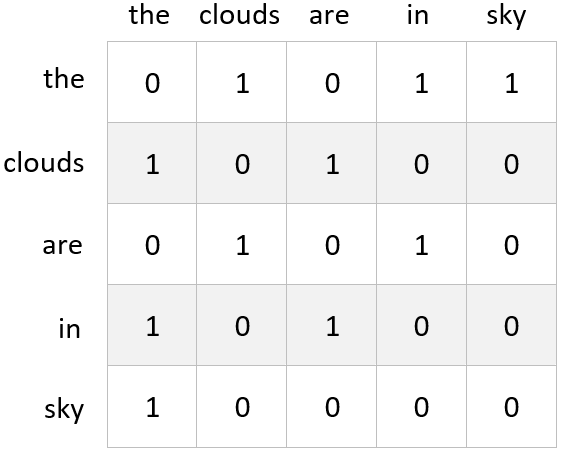
\includegraphics[width=0.3\textwidth]{Images/glovediagram.png}
	\label{GloVe Pipeline}
\end{center}

Given a corpus containing W tokens, a $W \times W$ matrix is constructed. The value in cell (x,y) denotes the frequency with which token \textit{x} has co-occurred with token \textit{y} within a fixed-size window. From this co-occurrence matrix, the probability of token \textit{x} co-occurring with token \textit{y} is given by the formula: \begin{center}
	$P_{co}\bigl( t_x | t_y\bigr) = \frac{C(t_y, t_x)}{C(t_y)}$
\end{center}
where $C(t_i, t_j)$ is the number of times token \textit{i} co-occurs with token \textit{j}.

The word meanings are encapsulated by the ratios of co-occurence probabilties, rather than the probabilities themselves.\\
\newpage
\noindent \textbf{Contextualised Word Embedding --}
Deep neural language models offer a more robust approach. Peters et al\ (2018) \cite{peters2018deep} introduced the \textit{ELMo} model, and showed that the addition of ELMo to existing models can markedly improve the state-of-the-art in a number of NLP tasks.\\

\begin{minipage}{0.4\textwidth}
	\begin{center}
		\textbf{Figure -:} ElMo model pipeline
	\end{center}
	\begin{center}
		\includegraphics[width=1\textwidth]{Images/elmo_diagram.png}
		\label{ElMo Model}
	\end{center}
\end{minipage} \hfill
\begin{minipage}{0.55\textwidth}
	ELMo utilises a bi-directional LSTM \textit{(long short-term memory)} model, concatenating the left-to-right and right-to-left LSTM in order to produce deep contextualised word representations. They are character based, therefore robust representations can be constructed for out-of-vocabulary tokens. However, rather than 'looking-up' pre-computed embeddings, ELMo generates them dynamically. Hence, it can disambiguate the sense of a word given the context in which it was found. These state-of-the-art contextualised embeddings are used in this project as the most advanced method of feature extraction.\\
\end{minipage}

\noindent \textbf{Experimentation with miscellaneous features --}
As supervised machine learning requires hand-crafted features to inform  predictions, we consider a number of hand-crafted features in addition to the vectors produced by the aforementioned vectorisation approaches. This includes lexical and sentiment features, as well as meta data where this is available as part of the original dataset. For example, the Sarcasm Amazon Review Corpus contains the number of stars in a review, and we can leverage this information as an additional feature. Features that can be shown to improve classifcation scores can be concatenated with our existing vectors (enrichment).\\

\noindent The following experiment is designed to answer the research question: \textit{Can we improve the solution by incorporating sentiment features?} We use a state-of-the-art model, the SentimentAnnotator \cite{socher2013recursive} by Stanford CoreNLP \cite{manning2014stanford}, in order to extract sentiment features from each of our datasets. The sentiment annotator assigns a discrete label between 0 (very negative) and 4 (very positive) to a snippet of text. For each instance in the dataset, we collect the sentiment values for each of the individual tokens, as well as the overall sentiment of the snippet. We contruct $ 1 \times 6 $ dimensional feature vectors, where values 0 - 4 show the distribution of sentiment classes for tokens in the snippet, and value 5 shows the overall sentiment label.\\

\noindent Example: \textit{"i love when my train is late!"}\\

\begin{tabular}{|p{3cm}||p{0.2cm}p{1cm}p{1cm}p{1cm}p{1cm}p{0.8cm}p{1cm}p{1cm}|}
	\hline 
	Tokens & i & love & when & my & train & is & late & !\\ 
	\hline 
	Sentiment Labels & 2 & 4 & 2 & 2 & 2 & 2 & 2 & 2\\ 
	\hline 
\end{tabular}
\vspace{10pt}

\begin{tabular}{|p{3.8cm}||p{1cm}|p{1cm}|p{1cm}|p{1cm}|p{1cm}|} 
	\hline 
	Sentiment Labels & {0} & {1} & {2} & {3} & {4}\\ 
	\hline 
	\textbf{Frequency} of tokens & 0 & 0 & 7 & 0 & 1\\ 
	\textbf{Proportion} of tokens & 0 & 0 & 0.875 & 0 & 0.125\\
	\hline  
\end{tabular}
\vspace{10pt}

{Overall sentiment}: 3.0\\
\indent {Feature vector}: [0.0, 0.0, 0.875, 0.0, 0.125, 3.0]\\


\subsection{Classification}
\noindent 
In this section, machine-learning and deep-learning classification models are considered. These algorithms are trained a set of rich features as outlined in the previous section.

\subsubsection{Machine Learning Models}
We experiment with five candidate machine learning classifiers, evaluating each of them when trained on four types of features. Each of these supervised models perform binary classification, where unseen samples are predicted to be sarcastic or non-sarcastic. A brief description of the models are provided below. 

\begin{enumerate}
	\item \textbf{K-Nearest Neighbours (KNN) --} The KNN classifier is a non-parametric model which uses lazy learning at the time of prediction. An unseen sample is assigned the most common class label amongst its k nearest neighbours, where k is a hyperparameter whose value is finetuned for each dataset.
	
	%As the only unsupervised algorithm used in this project, K-Means clustering partitions the set of unlabelled training data into K groups. K random cluster centres (centroids) are selected, then each data point is grouped together with the cluster at the nearest centroid. We use $K=2$ as we wish to divide the data into two groups. Although K-Means is intended to be a clustering algorithm, it can easilly be applied to classification problems if we assign the majority label to each cluster
	
	\item \textbf{Support Vector Machine (SVM) --} A hyperplane is drawn such that the positive and negative features are partitioned into two groups. The features at the shortest euclidean distance to the hyperplane are known as support vectors, and their distance from the hyperplane is known as the margin. An SVM attempts to maximise this margin in order to create a decisive boundary between the sarcastic and non-sarcastic data.
	
	\item \textbf{Na\"{i}ve Bayes Classifier --} This is a probabilistic model derived from Bayes theorem, where all features are assumed to be independent of one another. Commonly used in the document classification problem, we calculate ${P(Sarcastic | features)}$. This is  the probability of an outcome A (i.e. statement is sarcastic), given its feature vector, x. There are a number of variations of Na\"{i}ve Bayes - including Multinomial, Bernoulli and Gaussian. 

	\item \textbf{Logistic Regression --} A statistical model that aims to predict the likelihood of an event occuring given some previous data. It works with binary data, i.e. is the statement sarcastic or not. It is a more advanced approach than linear regression, which aims to model data using a linear equation.

	\item \textbf{Random Forest Classifier --}
	An ensemble learning method, the random forest classifier fits a number of decision tree classifiers on subsamples of the training set. The decision trees are fairly independent of one another, and this low correlation allows them to produce ensemble predictions that outperform their individual predictions. Where one model goes wrong, the others are able to contradict this incorrect prediction.
\end{enumerate}


\subsubsection{Deep Learning Models}
Deep learning classifiers do not need to use hand-crafted features used in supervised classifiers. We use Binary Cross-Entropy loss.

\paragraph{Recurrent Neural Networks --}
In a Recurrent Neural Network (RNN), prior inputs are used to inform future outputs. As in all neural networks, input vectors are modified by weighted nodes as they travel through the network. In a RNN, there is an additional hidden state which represents the context based on prior inputs, and is updated by inputs as they are fed through the network. This gives way to the interesting property that the same input could produce a different output depending on the previous inputs given to the RNN. In a vanilla RNN, the input and hidden state are simply propagated through a single tanh layer. However in a Long Short Term Memory model (LSTM), three gates are introduced, as well as a cell state, allowing an LSTM to better preserve long-term dependencies.\\

RNNs have been successfully applied to language-related tasks. Often, we may require more context than just the most recent surrounding text. The gap between the most relevant information needed to form a prediction can be very wide, if the relevent contextual information was given at the beginning of the paragraph. LSTMs are especially suited to processing sequential, or time-series, information such as text. This is due to the fact that RNNs have a 'memory', in that the input to the current step is the output from the previous step. However, they suffer from the vanishing gradient problem. This is where gradient values get smaller as it backtracks through lower layers, making it harder for the network to update weights and causing calculations to take longer. Recurrent Neural Networks are not very good at remembering long term dependencies, therefore in this instance we can use \textit{Long short-term memory (LSTM)} models \cite{hochreiter1997long} instead which are more effective at preserving long term dependencies.



\paragraph{Convolutional Neural Networks --}
A Convolutional Neural Network (CNN)\cite{lecun1998gradient} is a specialised form of neural network. They were popularised for their applications in computer vision, hence they are designed to be used with two-dimensional image data \cite{krizhevsky2012imagenet}, but have since been adapted for text-based classification tasks. CNNs consist of a few layers of convolutions with non-linear activation functions - they have fewer layers than typical neural networks, where each layer applies dfferent filters and combines their result. The convolution operation is very fast, therefore many convolutional layers can be used in a single network.

\begin{minipage}{0.35\textwidth}
	\begin{figure}[H]
		\begin{center}
		\textbf{Figure -}: $m \times n$ feature vector\\
		$
		\begin{bmatrix}
		w_{1,1} & w_{1,2} & ... & w_{1,N}\\
		w_{2, 1} & w_{2, 2} & ... & w_{2, N} \\
		\vdots & \vdots & \vdots & \vdots \\
		w_{M, 1} & w_{M, 2} & ... & w_{M, N} \\
		\end{bmatrix}
		$
	\end{center}
	\end{figure}
\end{minipage} \hfill
\begin{minipage}{0.6\textwidth}
	Each token in a sentence is represented independently by a fixed-size n-dimensional vector; as such, the sentence is represented by an $m \times n$ vector of feature weights, where m is the number of tokens in the sentence. This feature vector is used as input to the convolutional neural network. 
\end{minipage}

Convolutional layers compute the dot product of a kernel vector of k weights with k rows in the feature vector (representing a k-tokens in the input sentence), producing a new sequence of features. The convolution filter is repeatedly applied to overlapping sections of the matrix, and a max pooling operation is applied over each resulting feature map. Tokens in a sentence occur on a time axis, as the order that the tokens appear in gives rise to their meaning; hence, the filter slides downwards over the rows of the vector. Applying \textit{maximum pooling over time} produces a single output value following each convolution, such that the feature corresponding to a particular vector is the maximum activation in the feature map. Producing a fixed-size output matrix means that variable size sentences and variable size filters can be used to obtain features with the same output dimensions. This is especially useful for classification tasks, where the desired output is a fixed-sized vector indicating which class the input vector belongs to.



\section{Results}
\subsection{Evaluation Method}
\noindent This section discusses our approach to evaluating the successes and failures of the trained models. A simple approach is to use accuracy which refers to the proportion of data that is correctly labelled as either sarcastic or non-sarcastic. However, sarcasm is a minority class therefore on an unbalanced dataset we could achieve high accuracy by simply labelling every statement as non-sarcastic. In an attempt to mitigate against this, we instead form a conclusion based on the $F_{1}$ score i.e.\ the harmonic mean of precision and recall, where scores range from 0 (worst) to 1 (best). This metric has faced some criticism for giving equal weight to both precision and recall \cite{hand2018note}, therefore we consider both measures separately, as well as in combination.

\begin{align*}
\mbox{precision} &= \frac{\mbox{true positives}}{\mbox{true positives + false positives}}   &  \mbox{recall} &= \frac{\mbox{true positives}}{\mbox{true positives + false negatives}}
\end{align*}

\noindent In the domain of sarcasm detection, precision refers to the proportion of the classified-sarcastic data that is \textit{truly sarcastic} i.e.\ how many of the positives are true positives, and recall describes the proportion of the truly sarcastic data in the corpus that is \textit{classified} as such i.e.\ how many true positives are labelled as positives. \\

%this section presents the results of the solutions.  It should include information on experimental settings.  The results should demonstrate the claimed benefits/disadvantages of the proposed solutions.

\subsection{Feature Analysis}
\noindent We analyse the effectiveness of the hand-crafted features, sentiment, punctuation and topic modelling, on each of the three datasets. As the feature vectors are small, we use logistic regression for this task. We train three logistic regressors (one for each dataset) separately, using each feature type in isolation, then use 5-fold cross-validation to compute the $F_1$ scores of the trained models. This enables us to assess whether these features alone are indicative of sarcasm in different media types. We deem scores above 0.5 to be indicative of useful features, particularly for scores significantly greater than this baseline.


\begin{center}
	\textbf{Figure -}: $F_1$ score of logistic regression models trained on hand-crafted features
\end{center}

\begin{center}
	\begin{tabular}{|p{7cm}|p{1.8cm}|p{2.6cm}|p{1.6cm}|} 
		\hline
		& \multicolumn{3}{|c|}{\textbf{Feature Type}} \\
		\hline
		\textbf{Dataset} & \textbf{Sentiment} & \textbf{Punctuation} & \textbf{Topic} \\ [0.4ex] 
		\hline\hline
		News Headlines for Sarcasm Detection & 0.516 & 0.344 & 0.525\\ 
		\hline
		Sarcasm Amazon Review Corpus & 0.685 & 0.394 & 0.520\\ 
		\hline
		Pt\'a\v{c}ek et al. (2014) & 0.593 & 0.611 & 0.530\\
		\hline
	\end{tabular}
\end{center}

\noindent Our results show that sentiment features are indicative of sarcasm when extracted from the Sarcasm Amazon Review Corpus, however when extracted from the News Headlines for Sarcasm Detection, they were ineffective. To further examine this relationship between sarcasm and sentiment, we compute the mean proportion of tokens in each sentiment class for sarcastic and non-sarcastic instances. We then compute the absolute differences of these values between the sarcastic and non-sarcastic classes - the intuition being that it is simpler for a classifier to separate samples where there is a clearer distinction between the expected features of each class. Hence, where the absolute difference in the mean proportion of tokens between sarcasm classes is higher, a classifier is better able to correctly annotate samples. A visualisation of these results is given in the figure below.

\begin{minipage}{0.4\textwidth}
	\begin{figure}[H]
		\begin{center}
			\textbf{Figure -:} Absolute differences\\
			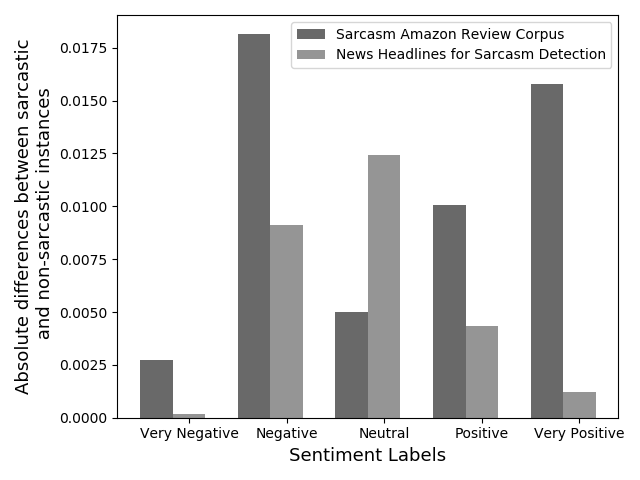
\includegraphics[width=0.95\textwidth]{Images/absolute_differences.png}
			\label{Sarcasm Amazon Review Corpus}
		\end{center}
	\end{figure}
\end{minipage} \hfill
\begin{minipage}{0.6\textwidth}
	For the Sarcasm Amazon Review Corpus, within most sentiment classes there is a greater difference in the proportion of tokens for non-sarcastic and sarcastic instances. This indicates that sarcastic and non-sarcastic instances are easier to distinguish, given that their sentiment compositions are more distinct. The News Headlines for Sarcasm Detection results displays the opposite, and this explains why the logistic regression classifier trained on this data achieved an $F_1$  score of only 0.515, as the features for each class are very similar.
\end{minipage}


%\begin{figure}[htp]
%	\centering
%	\textbf{Figure -:} Mean proportion of tokens in each sentiment class
%%	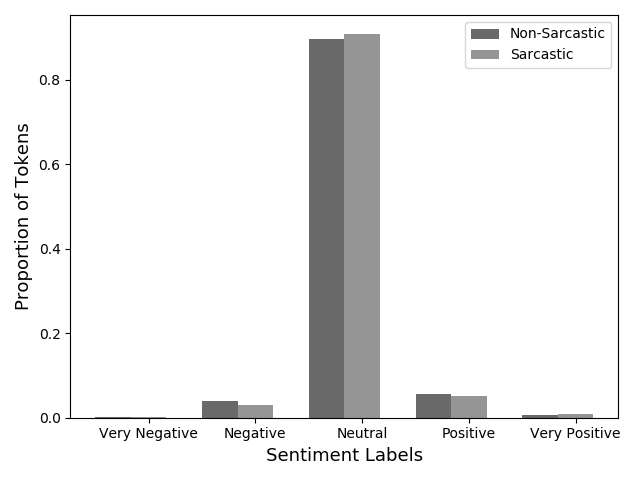
\includegraphics[width=.5\textwidth]{Images/NHSD_sentimentlabels.png}\hfill
%	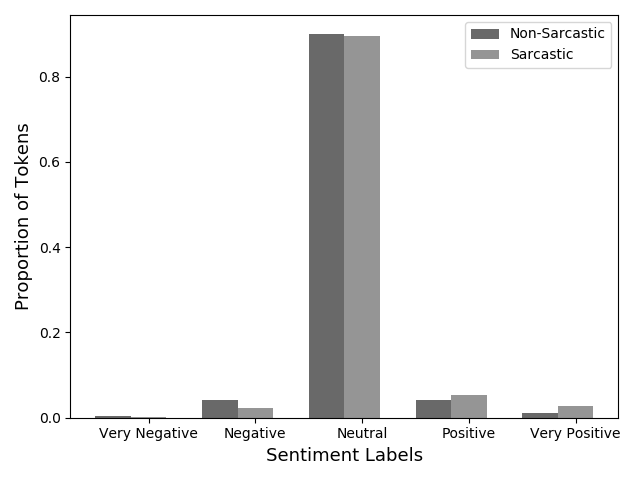
\includegraphics[width=.5\textwidth]{Images/SARC_sentimentlabels.png}\hfill
%	\label{fig:figure3}
%\end{figure}

\subsection{Machine Learning Experimentation}



\noindent We train a range of classifiers independently on each of the three datasets, and provide the results of this experimentation in the following subsections. The $F_{1}$ scores of the trained models are provided to 3 significant figures, and the score of the best-performing model is highlighted for clarity. Each classifier is trained on four types of vectors, Bag of Words, TF-IDF, GloVe and ElMo as outlined in the solution.\\

We also experimented with an unsupervised model - K-Means clustering where the majority label of each cluster was assigned, however, the results were very poor.



\noindent \textbf{Experimental Settings --} For the machine learning experiments, 5-fold cross validation was employed to ensure reproducability and consistency of results. We allocate 80\% of data to the training set, and the remaining 20\% to the testing set for each of the five folds. For the K-nearest neighbor classifier, K = 5 was found to be the greatest balance between computational cost and noise mitigation.



%\subsubsection{News Headlines for Sarcasm Detection}

\begin{center}
	\textbf{Figure -}: $F_1$ scores of Machine Learning classifiers on the \\\textit{News Headlines for Sarcasm Detection} dataset
\end{center}

\begin{center}
	\begin{tabular}{ |p{4.7cm}||p{1.2cm}|p{1.5cm}|p{1.2cm}|p{1.2cm}|  }
		\hline
		& \multicolumn{4}{|c|}{\textbf{Vector}} \\
		\hline
		\textbf{Model Architechture}& \textbf{BOW} & \textbf{TF-IDF} & \textbf{GloVe} & \textbf{ElMo}\\
		\hline\hline
		Support Vector Machine   & 0.714    & 0.718 &   0.732 & 0.844\\
		Logistic Regression &   0.721 & 0.712   & 0.732 & \textbf{0.846}\\
		Random Forest Classifier &0.530 & 0.643 &  0.754 & 0.797\\
		Gaussian Naive Bayes  & 0.662  & 0.649&  0.703 &0.640\\
		K-Nearest Neighbours& 0.569  & 0.483   & 0.709 & 0.788\\
		\hline
	\end{tabular}
\end{center}

\begin{center}
	\begin{tabular}{ |p{9cm}||p{2cm}|  }
		\hline
		\textbf{Model Architechture}&  \textbf{$\mathbf{F_1}$ Score}\\
		\hline\hline
		Logistic Regression + ElMo + Sentiment   & 0.846\\
		Logistic Regression + ElMo + Punctuation & 0.847\\
		Logistic Regression + ElMo + Topic   & 0.847\\
		Logistic Regression + ElMo + Topic + Punctuation   & 0.847\\
		\hline
	\end{tabular}
\end{center}


%\subsubsection{Sarcasm Amazon Review Corpus}

\begin{center}
	\textbf{Figure -}: $F_1$ scores of Machine Learning\\ classifiers on the \textit{Sarcasm Amazon Review Corpus}
\end{center}

\begin{center}
	\begin{tabular}{ |p{4.7cm}||p{1.2cm}|p{1.5cm}|p{1.2cm}|p{1.2cm}|  }
		\hline
		  & \multicolumn{4}{|c|}{\textbf{Vector}} \\
		\hline
		\textbf{Model Architechture}& \textbf{BOW} & \textbf{TF-IDF} & \textbf{GloVe} & \textbf{ElMo}\\
		\hline\hline
		Support Vector Machine   & 0.736    & 0.775 &   0.700 & 0.800\\
		Logistic Regression &   0.745 & 0.748   & 0.713 & \textbf{0.809}\\
		Random Forest Classifier &0.525 & 0.487 &  0.669 & 0.727\\
		Gaussian Naive Bayes  & 0.625  & 0.621 &  0.416 & 0.666\\
		K-Nearest Neighbours & 0.476  & 0.607   & 0.561 & 0.685\\
		\hline
	\end{tabular}
\end{center}

\begin{center}
	\begin{tabular}{ |p{9cm}||p{2cm}|}
		\hline
		\textbf{Model Architechture}&  \textbf{$\mathbf{F_1}$ Score}\\
		\hline\hline
		Logistic Regression + ElMo + Sentiment   & 0.830\\
		Logistic Regression + ElMo + Punctuation & 0.809\\
		Logistic Regression + ElMo + Topic   & 0.811\\
		Logistic Regression + ElMo + Sentiment + Topic & 0.811\\
		\hline
	\end{tabular}
\end{center}

%\subsubsection{Pt\'a\v{c}ek et al. (2014) Dataset}

\begin{center}
	\textbf{Figure -}: $F_1$ scores of Machine Learning\\ classifiers on the \textit{Pt\'a\v{c}ek et al. (2014) dataset}
\end{center}

\begin{center}
	\begin{tabular}{ |p{4.7cm}||p{1.2cm}|p{1.5cm}|p{1.2cm}|p{1.2cm}|  }
		\hline
		& \multicolumn{4}{|c|}{\textbf{Vector}} \\
		\hline
		\textbf{Model Architechture}& \textbf{BOW} & \textbf{TF-IDF} & \textbf{GloVe} & \textbf{ElMo}\\
		\hline\hline
		Support Vector Machine   & 0.713    & 0.724 &   0.635 & 0.754\\
		Logistic Regression &   0.742 & 0.748 & 0.630 & \textbf{0.762}\\
		Random Forest Classifier &0.723 & 0.715 &  0.645 & 0.735\\
		Gaussian Naive Bayes  & 0.681  & 0.675&  0.594 &0.684\\
		K-Nearest Neighbours & 0.557  & 0.346   & 0.607 & 0.716\\
		\hline
	\end{tabular}
\end{center}

\begin{center}
	\begin{tabular}{|p{9cm}||p{2cm}| }
		\hline
		\textbf{Model Architechture}&  \textbf{$\mathbf{F_1}$ Score}\\
		\hline\hline
		Logistic Regression + TF-IDF + Sentiment   & 0.763\\
		Logistic Regression + TF-IDF + Punctuation & 0.762\\
		Logistic Regression + TF-IDF + Topic   & 0.763\\
		Logistic Regression + TF-IDF + Sentiment + Topic & 0.764\\
		\hline
	\end{tabular}
\end{center}



%
%\begin{center}
%	\textbf{Figure -}: Results of Machine Learning Classifiers on the Sarcasm Amazon Review Corpus
%\end{center}
%\begin{center}
%	\begin{tabular}{p{8cm}p{2cm}}
%		\hline
%		\textbf{Model architecture} & \textbf{$F_{1}$ Score}\\
%		\hline\hline
%		GloVe + Support Vector Machine & 0.739\\
%		\hline
%		GloVe + Logistic Regression & 0.730\\
%		\hline
%		GloVe + Random Forest Classifier & 0.644\\
%%		\hline
%		GloVe + Gaussian Na\"{i}ve Bayes & 0.415\\
%		\hline
%	\end{tabular}\\
%\end{center}



%This section should be between 2 to 3 pages in length.

\newpage
\subsection{Deep Learning Experimentation}
\noindent Each deep learning model is trained separately on each of the three datasets, using glove vectors and elmo vectors. Sparse feature representations such as tf-idf and bag of words are not used as

\subsubsection{Experimental Settings}
The upper-bound on the number of epochs is 300, although this is seldom reached due to the use of the Early Stopping callback function. The patience is set to 20, and this is the number of epochs for which no improvement can be seen before the training is prematurely terminated. However, setting the patience too low can hamper a model that plateaus for a while before continuing to improve.

\begin{enumerate}
	\item \textbf{Early stopping --} Training is interrupted when the validation loss stops declining, using thins to determine the appropriate number of epochs.
	\item \textbf{Model Checkpointing --} We track and save the weights of the best performing model during training; the model with the lowest validation loss.
\end{enumerate}

Preliminary experimentation showed that the training process on the Sarcasm Amazon Review corpus was very unstable as this dataset is small. Results varied widely, and model scores were significantly lower. We augment this particular dataset using a synonym replacement strategy, whereby for each instance of the dataset, a new instance is added. This is a modified version of the 


\begin{center}
	\textbf{Figure -}: $F_1$ scores of Deep Learning classifiers on the \\\textit{News Headlines for Sarcasm Detection} dataset
\end{center}

\begin{center}
	\begin{tabular}{|p{4.7cm}||p{1.2cm}|p{1.5cm}|}
		\hline
		& \multicolumn{2}{|c|}{\textbf{Vector}} \\
		\hline
		\textbf{Model Architechture}& \textbf{GloVe} & \textbf{ElMo}\\
		\hline\hline
		CNN   & 0.823   & \\
		LSTM &   0.865 & 0.\\
		Bi-directional LSTM & 0.864 & 0.\\
		Vanilla RNN &0.817 & 0.\\
		Vanilla GRU &0.852 & 0.\\
		\hline
	\end{tabular}
\end{center}


\begin{center}
	\textbf{Figure -}: $F_1$ scores of Deep Learning\\ classifiers on the \textit{Sarcasm Amazon Review Corpus}
\end{center}

\begin{center}
	\begin{tabular}{ |p{4.7cm}||p{1.2cm}|p{1.5cm}|  }
		\hline
		& \multicolumn{2}{|c|}{\textbf{Vector}} \\
		\hline
		\textbf{Model Architechture}& \textbf{GloVe} & \textbf{ElMo}\\
		\hline\hline
		CNN   & 0.  & 0.\\
		LSTM &   0. & 0.\\
		Bi-directional LSTM &0. & 0.\\
		\hline
	\end{tabular}
\end{center}



\begin{center}
	\textbf{Figure -}: $F_1$ scores of Deep Learning\\ classifiers on the \textit{Pt\'a\v{c}ek et al. (2014) dataset}
\end{center}

\begin{center}
	\begin{tabular}{ |p{4.7cm}||p{1.2cm}|p{1.5cm}|  }
		\hline
		& \multicolumn{2}{|c|}{\textbf{Vector}} \\
		\hline
		\textbf{Model Architechture}& \textbf{GloVe} & \textbf{ElMo}\\
		\hline\hline
		CNN   & 0.  & 0.\\
		LSTM &   0. & 0.\\
		Bi-directional LSTM &0. & 0.\\
		\hline
	\end{tabular}
\end{center}

\newpage


\section{Evaluation}
In the following section, we analyse the effectiveness of the solution, discussing its strengths and weaknesses and evaluating to what extent it satisfies the research questions and deliverables.

\subsection{Solution Strengths}
We found that sentiment features can be useful predictors of sarcasm in \textit{some} forms of media. This may be due to the fact that sarcasm must be more overt in product reviews in order to mock the product, rather than the subtle, more contextualised instances in News Headlines.



\subsection{Solution Limitations}
It was only feasible to evaluate a small range of online media types, however surveying a broader range of media types could give us a wider perspective of sarcasm in online media.


\subsection{Lessons learnt}
We learned that 


\subsection{Project organisation and approach}




%This section should between 1 to 2 pages in length.

\section{Conclusions}
In terms of satisfying the objectives, this project was an overall success. With an interactive console, it may be useful to individuals who struggle to detect sarcasm in their daily-life, or for the industrial applications of enhanced opinion mining.

The main contributions of this project are as follows: sentiment features are combined with state-of-the-art vectorisation approaches. 

For future work, it would be interesting to explore the use of sarcasm in a wider variety of media types, and to extend support to additional non-English languages. Exploring the use of transfer learning with Transformers (BERT) may also produce interesting results.


%This section summarises the main points of this paper.  Do not replicate the abstract as the conclusion.  A conclusion might elaborate on the importance of the work or suggest applications and extensions.  This section should be no more than 1 page in length.

%The page lengths given for each section are indicative and will vary from project to project but should not exceed the upper limit.  A summary is shown in Table \ref{summary}.

\begin{table}[htb]
\centering
\caption{SUMMARY OF PAGE LENGTHS FOR SECTIONS}
\vspace*{6pt}
\label{summary}
\begin{tabular}{|ll|c|} \hline
& \multicolumn{1}{c|}{\bf Section} & {\bf Number of Pages} \\ \hline
I. & Introduction & 2--3 \\ \hline
II. & Related Work & 2--3 \\ \hline
III. & Solution & 4--7 \\ \hline
IV. & Results & 2--3 \\ \hline
V. & Evaluation & 1-2 \\ \hline
VI. & Conclusions & 1 \\ \hline
\end{tabular}
\end{table}

\newpage
\bibliography{FinalPaper}


\end{document}